\LectureAnswerSection

\begin{drillsolution}{c1d1}\textbf{分别计算三个因子的变化贡献}\par\nobreak
乘积求导时，每次只改变一个因子，其余两个暂时保持原值，再把三次贡献相加。也可先令 $u=x\sin x$，由 $u'=\sin x+x\cos x$ 求得 $f'=\e^x u'+\e^x u$；两种分组应给出同一结果。切线还须同时经过题设点，因而不能只报告斜率。

图 \ref{c1d1q} 中每个因子都有变化，故
\[
 f'=\e^x\sin x+x\e^x\cos x+x\e^x\sin x
 =\e^x[(1+x)\sin x+x\cos x].
\]
\fig{c1d1s}{三条求导路径与零点的水平切线}{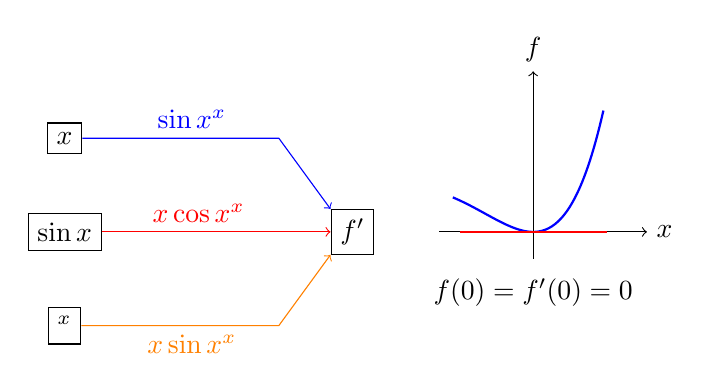
\begin{tikzpicture}[scale=.85]
\node[draw](a)at(0,1.4){$x$};\node[draw](b)at(0,0){$\sin x$};\node[draw](c)at(0,-1.4){$\e^x$};\node[draw](d)at(4.3,0){$f'$};
\draw[->,blue](a.east)--(3.2,1.4)--(d.north west);\node[blue,above]at(1.9,1.4){$\sin x\e^x$};
\draw[->,red](b.east)--(d.west);\node[red,above]at(2,0){$x\cos x\e^x$};
\draw[->,orange](c.east)--(3.2,-1.4)--(d.south west);\node[orange,below]at(1.9,-1.4){$x\sin x\e^x$};
\begin{scope}[xshift=7cm]\draw[->](-1.4,0)--(1.7,0)node[right]{$x$};\draw[->](0,-.4)--(0,2.4)node[above]{$f$};
\draw[blue,thick,domain=-.8:.7,samples=80]plot({1.5*\x},{2*\x*sin(\x r)*exp(\x)});\draw[red,thick](-1.1,0)--(1.1,0);\node at(0,-.9){$f(0)=f'(0)=0$};\end{scope}
\end{tikzpicture}}



\par\medskip\Needspace{4\baselineskip}\noindent\textbf{同时确定切线斜率与切点}\par\nobreak
图 \ref{c1d1s} 左侧的三条路径分别给出一个因子的变化贡献，相加才是总变化率；右侧红线用于核对零点切线。代入 $x=0$ 时 $\sin0=0,\cos0=1,\e^0=1$，得到 $f(0)=0$、$f'(0)=0$。切线的一般方程为 $y-f(0)=f'(0)(x-0)$，所以本题为 $y=0$。又因 $\sin x\sim x,\e^x\to1$，有 $f(x)\sim x^2$，与水平切线相符。



\par\medskip\Needspace{4\baselineskip}\noindent\textbf{用导数定义核验零点斜率}\par\nobreak
零点处还可直接用定义作独立检查，而不再次使用乘积法则。由 $f(0)=0$，有
\[f'(0)=\lim_{h\to0}\frac{h\sin h\e^h}{h}
       =\lim_{h\to0}\sin h\e^h=0.\]
定义法只检验这一点的局部变化，前面的乘积法则则给出整个可导区间的表达式；二者所得零点斜率一致。
\end{drillsolution}
\begin{drillsolution}{c1d2}\textbf{先检查函数在零点是否连续}\par\nobreak
这里要分别回答函数值是否连续与差商是否有唯一极限。先将左右函数值与零点定义比较，再计算左右差商，次序不能倒置。$g$ 的正、负两支虽然表达式不同，零点导数仍可能相同；这个例子说明分段形式本身并不意味着不可导。

图 \ref{c1d2q} 两侧都趋于零，且 $f(0)=0$，所以连续。

\par\medskip\Needspace{4\baselineskip}\noindent\textbf{比较绝对值函数的左右差商}\par\nobreak
求零点导数时，$h>0$ 的差商为 $h/h=1$，$h<0$ 时为 $(-h)/h=-1$，两侧不同，故不可导。

\par\medskip\Needspace{4\baselineskip}\noindent\textbf{检查乘上横坐标后斜率怎样改变}\par\nobreak
对 $g$，有 $g(x)=x^2$（$x>0$）和 $g(x)=-x^2$（$x<0$），两侧也都趋于 $g(0)=0$。其零点差商为 $h|h|/h=|h|\to0$，所以可导且 $g'(0)=0$。
\fig{c1d2s}{乘以横坐标后，零点成为水平切点}{\begin{tikzpicture}[scale=.9]
\draw[axis](-1.8,0)--(1.9,0)node[right]{$x$};\draw[axis](0,-1.6)--(0,1.7)node[above]{$g$};
\draw[blue,domain=-1.2:1.2,samples=60]plot(\x,{\x*abs(\x)});
\draw[guide](-1,0)--(1,0);\fill(0,0)circle(1.5pt);
\end{tikzpicture}}
图 \ref{c1d2s} 的两侧切线在零点一致。区间内 $g'(x)=2|x|$，与零点的导数连续衔接；这不是由函数连续本身推出的，而是差商计算的结果。
\end{drillsolution}
\begin{drillsolution}{c1d3}\textbf{把几何路径与时间规律结合}\par\nobreak
图中的几何曲线没有包含行进快慢。必须先把 $x=ut$ 代入，或用链式法则把对 $x$ 的变化率转换成对 $t$ 的变化率。由于水平运动匀速，$\ddot x=0$；竖直坐标仍随时间二次增长，因此竖直加速度并不为零。

图 \ref{c1d3q} 的几何式给出路径，时间式给出走过路径的方式。代入得 $y=\beta u^2t^2$，故
\[
 \bm v=(u,2\beta u^2t),\qquad \bm a=(0,2\beta u^2).
\]
\fig{c1d3s}{速度沿切线，加速度沿竖直方向}{\begin{tikzpicture}
\draw[world,domain=0:3,samples=40]plot(\x,{.22*\x*\x});\coordinate(P)at(2,.88);\fill(P)circle(2pt)node[below]{$P$};
\draw[force,blue](P)--++(.9,.792)node[right]{$\bm v$};\draw[force,red](P)--++(0,1.3)node[above]{$\bm a$};
\end{tikzpicture}}


\par\medskip\Needspace{4\baselineskip}\noindent\textbf{沿图中方向核对加速度与量纲}\par\nobreak
图 \ref{c1d3s} 中 $\bm a$ 没有水平分量，因为 $\dot x=u$ 为常数。竖直分量的逐步计算为
$\dot y=2\beta x\dot x=2\beta u^2t$，
$\ddot y=2\beta(\dot x^2+x\ddot x)=2\beta u^2$。
$y''(x)=2\beta$ 的量纲为逆长度，$\ddot y$ 的量纲为加速度；中间的 $\dot x^2=u^2$ 正是改变自变量时产生的因子，不能省去。
\end{drillsolution}
\begin{drillsolution}{c1d4}\textbf{在零点处统一三角函数的自变量}\par\nobreak
前两个极限都先化为已知的 $\sin z/z$ 型。第一式补出并约去常数三，保证分子、分母具有同一个趋零变量；第二式先用 $1-\cos2x=2\sin^2x$，避免直接把两个趋零量分别置零。最后一式考察无穷远行为，应将分子、分母同除以 $x$，再利用正弦与余弦有界。

结合图 \ref{c1d4q} 的趋近方向，
\[
 \frac{\sin3x}{x}=3\frac{\sin3x}{3x}\to3,\qquad
 \frac{1-\cos2x}{x^2}=2\left(\frac{\sin x}{x}\right)^2\to2.
\]
\fig{c1d4s}{正弦与余弦的修正项都落在逐渐收窄的包络内}{\begin{tikzpicture}

\draw[axis](0,0)--(7.3,0)node[right]{$x$};\draw[axis](0,-1.3)--(0,1.4)node[above]{比值};
\fill[gray!10]plot[domain=1:7,samples=60](\x,{1/\x})--plot[domain=7:1,samples=60](\x,{-1/\x})--cycle;
\draw[guide,domain=1:7,samples=70]plot(\x,{1/\x});\draw[guide,domain=1:7,samples=70]plot(\x,{-1/\x});
\draw[blue,thick,domain=1:7,samples=90]plot(\x,{sin(\x r)/\x});\draw[red,thick,domain=1:7,samples=90]plot(\x,{cos(\x r)/\x});
\node[above]at(5.8,.5){$1/x$};\node[below]at(5.8,-.5){$-1/x$};
\node[blue]at(2.2,1.6){$\sin x/x$};\node[red]at(5,1.6){$\cos x/x$};
\end{tikzpicture}}


\par\medskip\Needspace{4\baselineskip}\noindent\textbf{在无穷远处控制有界修正项}\par\nobreak
图 \ref{c1d4s} 的有界性使
$\displaystyle\frac{x+\sin x}{2x-\cos x}
=\frac{1+\sin x/x}{2-\cos x/x}\to\boxed{1/2}$。
分母趋于 $2$，满足商的极限法则的非零条件。
\end{drillsolution}
